\chapter{结合RFM与核密度估计的气井分类算法}
在气井开采初期,气井一经投入使用就会打破气藏的静态平衡,诸如产量、压力和产物性质等关键参数便会随之变动。随着开采活动的进行,气水关系会愈加错综复杂。产水量将持续攀升,
低压井和产水井的数量不断增长,不同气井之间的差异会日益增大。这些因素会进一步增加气井的生产管理难度。为提高管理效能,企业需利用历史产量数据对气井进行有效分类。将
表现出相似生产特性的气井进行归类和分析,以帮助揭示它们的共同生产模式。使得企业能够迅速评估气井的生产状况,掌握关键生产特征,进而及时规划出针对性强的管理策略和治
理行动,以确保气井的顺畅运作。本章使用了结合RFM与核密度估计的气井分类算法,根据根据气井的数据特征,对气井进行分类。首先对企业提供的报表数据进行整理和清洗,去除掉
报表中的冗余数据并将需要的信息批量提取出来。在获取了相应的气井信息后,使用结合RFM与核密度估计的气井分类算法来对气井进行分类,并在第四章通过实验验证经过分类后再对气井
进行预测效果会更好。
\section{问题分析}
企业气田的地质条件十分复杂,是典型的“低渗透、低压力、低丰度”气田。其单井产量小、压降速率快,随着气田不断进行规模开发,单井井数逐年增加,集气站也在不断的增大。
随着开采活动的不断进行,间歇井(气井按照固定的开关制度进行生产的气井)数量的也在逐步递增。气井在开采过程中,产量会随着井底污染、地层压力、地层渗透率、地层有效厚度
等的变化。不同气井之间的特征差异较大,需要通过合理的方式对气井进行分类。本文中初步想法是根据企业所提供报表数据,使用普通聚类算法如KMeans或者时间序列聚类算法如K-Shpae等对气井进行无监督分类。然而使用
这类聚类算法后发现该方法不具有稳定性,每次分类结果都不尽相同,无法达到向企业交付的标准。同时,对数据分布进行可视化展示以后,发现数据不是成团分布
,数据之间差异不大,不能简单地使用普通聚类算法。而采用K-Shpae进行时间序列聚类之后,发现不同类别之间无法提取出比较相似的特征,同一类别较为凌乱,
不能作为企业对气井分类的标准。经过分析发现普通的时间序列聚类算法大多是对过去时间序列的形状进行聚类,通过对K-Shape实验的数据结果\cite{Kshapeexperiment}
分析可以发现,其对于具有相似形状或模式的时间序列会有更好的分类效果,例如心跳、交通等具有相似周期性、趋势或季节性模式的时间序列。本文气井的时间序列没有
明显规律,因此其聚类效果较差。经过探索并依赖企业专家的领域知识,本文启发式的采用基于RFM\cite{birant2011data}评价参数结合核密度估计的方式来对气井进行分类。RFM模型是一种用于分析
客户价值和客户创收能力的方法,常用于数据库营销和直接营销中。将RFM模型应用于气井分类,可以充分挖掘气井的潜在价值。通过RFM模型来选取相应的参数,再根据数据的密度特征
选取相应的阈值,通过特征二值化的方法来对气井进行分类。
\section{问题描述}
在气井分类的问题的目标是将具有相似特征的气井分为一组,以帮助企业根据气井的特征更好地进行管理。此研究问题是提供某一气井相关数据,
确定其所属类别。问题的输入是气井的相关信息,单个数据可以表示为$x_i = \{x_{i1}, x_{i2}, \ldots, x_{iN}\}$,N表示特征数,输入数据集
$\mathbf{X} = \{X_{1}, X_{2}, \ldots, X_{m}\}$,m表示数据量的大小,输出是气井类别,将气井输出集表示为$\mathbf{Y}$,问题可以形式化为
求$\mathbf{X}$到$\mathbf{Y}$的一个映射$f$:$X \rightarrow Y$。
\section{算法框架}
\subsection{算法流程}\
\label{sec:K-Shapeprocess}
根据前文所述,传统的聚类方法以及基于时间的聚类方法在气井分类问题中效果较差,需要探寻一种合适的分类方法来对气井进行科学的分类。这其中的难点主要是
如何选取合适的分类模型以及合适的特征来对气井进行分类。本文采用在营销分析时常用的数据挖掘工具RFM模型来评估气井的价值。具体流程如图\ref{fig:wellcla}所示。
\begin{figure}
    \centering
    % Requires \usepackage{graphicx}
    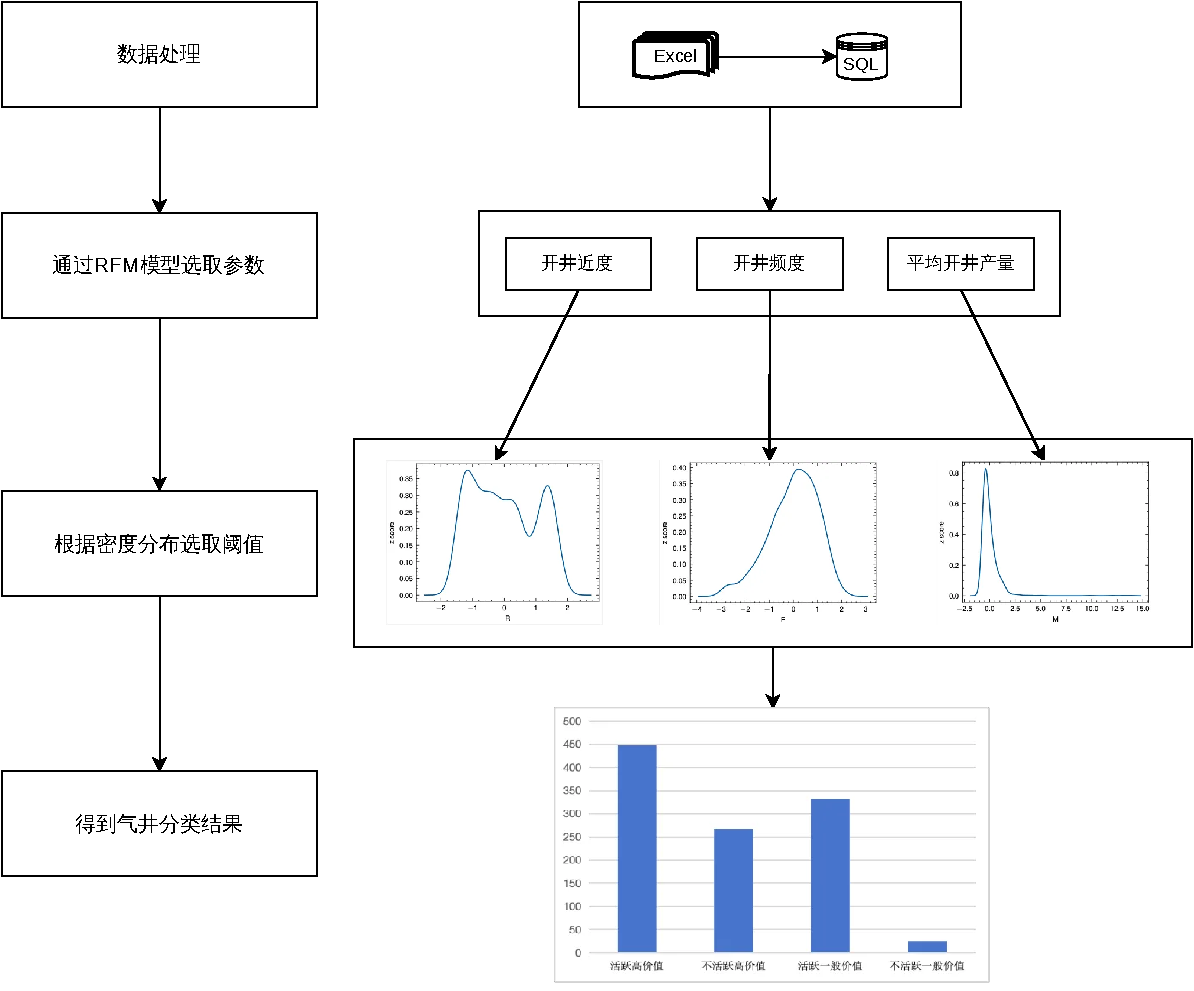
\includegraphics[width=.8\linewidth]{figure/气井分类框架图.vision.pdf}
    \caption{结合RFM与核密度估计的气井分类算法框架图}
    \label{fig:wellcla}
\end{figure}
在进行气井数据分析的初始阶段,难题在于如何从原始报表中提取准确信息,该报表数据错综复杂且杂乱无章。为了将这些数据转化为一份规范化的报表,首先需要对原始数据进行细致的清理和整理工作。这一过程不仅涉及去除无关或重复的数据,还包括标准化数据格式和校正数据不一致性,以确保最终报表的数据质量和可靠性。

在构建规范化的数据框架之后,本文进一步利用RFM(Recency, Frequency, Monetary)模型作为分析工具来评估气井的生产性能特征。在本研究场景中,RFM模型的参数需要根据气井的生产数据特性进行相应的调整和定义。这些参数的选取和优化对于后续分析的准确性和实用性至关重要。

紧接着,本文需要对选定的参数进行密度分布分析,以根据其分布来选取合理的划分阈值。通过核密度估计(KDE)方法,可以对气井参数的分布情况进行可视化解读,从而识别出关键的数据特征和潜在的生产趋势。

最终本文利用得到的密度分布信息进行特征二值化处理。通过这种方法,本文可以有效地将气井划分为四类,为进一步的分析和决策提供支持。通过这一系列系统的数据处理和分析步骤,能够深入理解并分类气井的生产效率,为后续的资源分配和优化策略提供坚实的数据基础。
\subsection{数据处理}
\label{cha:data}
原始数据集由单井日报文件组成,涵盖了从2012年8月3日至2022年8月15日的时间跨度。这些数据以Excel格式存储,其中一个月的数据被归纳于一张多工作表的Excel文件中,一年由12张此类文件构成。每张多工作表文件包括了该月内每天的数据,每天的数据记录在单独的Excel工作表中。

每张工作表中的信息包括所属井丛、井号、配产、生产时间(包括日累和月累,月累数据自2014年4月起引入)、油压、套压(自2016年9月起引入)、井口温度、注醇量(以井丛计)、产气量(包括日产、月累、年累及历年年累)、投产日期及备注(包括开关井信息等)。

在进行数据的批量读取和处理前,需要对这些报表按照不同的格式进行分类,考虑的因素包括不同的表头、报表的组织形式、日期记录的格式,以及剔除一些非必要的表格,例如某些含有总结性信息的表格,这些信息可能会干扰批量处理。以2012年的数据为例,其格式相对杂乱,8月和9月的
数据以单独的Excel文件记录每一口井的日报,而10月至12月的数据则分别存储在三个不同的Excel文件中,每个文件包含相应月份的数据。
如表\ref{tab:examplewell}展示了气井包含信息示例。
% \begin{table}[H]
%     \renewcommand{\arraystretch}{1.5}
%     \centering
%     \caption{气井信息示例表}
%     \label{tab:examplewell}
%     \begin{tabularx}{\textwidth}{|l|Y|Y|Y|Y|}
%         \hline
%         名称 & 序号 & 丛式井 & 井号 & 配产($10^4 m^3/d$) \\
%         \hline
%         样例 & 1 & 013井丛 & AA26EF-01 & 2.3 \\
%         \hline
%         \multirow{2}{*}{名称} & \multicolumn{2}{c|}{生产时间(h)} & \multirow{2}{*}{井口压力 ($MPa$)} & \multirow{2}{*}{井口套压 ($MPa$)} \\
%         \cline{2-3} & 日产时间 & 月累 & & \\
%         \hline
%         样例 & 16.00 & 600.00 & 1.73 & 4.09 \\
%         \hline
%         \multirow{2}{*}{名称} & \multirow{2}{*}{井口温度($^\circ$C)} & \multicolumn{3}{c|}{注醇量(L)} \\
%         \cline{3-5} & & 日注醇 & 月累 & 年累 \\
%         \hline
%         样例 & 12.20 & 720 & 18000 & 39700 \\
%         \hline
%         \multirow{2}{*}{名称} & \multicolumn{4}{c|}{产气量($10^4 m^3$)} \\
%         \cline{2-5} & 日产 & 月累 & 年累 & 历年年累 \\
%         \hline
%         样例 & 1.0754 & 31.2484 & 104.4155 & 2253.7500 \\
%         \hline
%         名称 & 投产日期 & 生产方式 & 备注 & 井口油压 ($MPa$) \\
%         \hline
%         样例 & 2020/11/16 & VS & 低压\_调峰井 & 3.44 \\
%         \hline
%     \end{tabularx}
% \end{table}

\begin{table}[H]
    \centering
    \caption{气井信息示例表}
    \label{tab:examplewell}
    \begin{tblr}{
        width = \textwidth,
        colspec = {|X[l]|X[c]|X[c]|X[c]|X[c]|},
        hlines, vlines,
        columns = {valign=m},
        rows    = {halign=c, font=\renewcommand{\arraystretch}{1.5}},
        cell{3}{1} = {r=2}{c},
        cell{3}{2} = {c=2}{},
        cell{6}{1} = {r=2}{c},
        cell{6}{2} = {r=2}{c},
        cell{6}{3} = {c=3}{},
        cell{9}{2} = {c=4}{},
        cell{9}{1} = {r=2}{c},
    }
        名称 & 序号 & 丛式井 & 井号 & 配产($10^4 m^3/d$) \\
        样例 & 1 & 013井丛 & AA26EF-01 & 2.3 \\
        名称 & 生产时间(h) & & 井口压力 ($MPa$) & 井口套压 ($MPa$) \\
        & 日产时间 & 月累 & & \\
        样例 & 16.00 & 600.00 & 1.73 & 4.09 \\
        名称 & 井口温度($^\circ$C) & 注醇量(L) & & \\
        & & 日注醇 & 月累 & 年累 \\
        样例 & 12.20 & 720 & 18000 & 39700 \\
        名称 & 产气量($10^4 m^3$) & & & \\
        & 日产 & 月累 & 年累 & 历年年累 \\
        样例 & 1.0754 & 31.2484 & 104.4155 & 2253.7500 \\
        名称 & 投产日期 & 生产方式 & 备注 & 井口油压 ($MPa$) \\
        样例 & 2020/11/16 & VS & 低压\_调峰井 & 3.44 \\
    \end{tblr}
\end{table}


经过与企业专家沟通,本文选取了日期、集气站号、井序号、日产时间、井口压力(油压)、套压、井口温度、日产量和投产时间等关键指标。其中套压数据的记录是从2016年9月开始的,这个时间点之前的数据中不包括套压信息。

在批量处理和读取原始数据的过程中,首先要去除每张Excel表中的冗余信息,这包括无关的汇总信息、非结构化的备注或者其他非目标数据列。随后,从每张表中提取出所需的关键列,这一步骤将会生成每个单井每日的数据记录,每天的记录将被整理并存储在一个单独的CSV格式文
件中。处理完整个时间范围后,生成了3664个此类文件,每个文件代表一个日报的数据集,覆盖从2012年8月3日至2022年8月15日的时间段。

接下来,将这些单日数据集进行统一处理以建立一个完整的数据集,该过程包括填充空值、进行数据格式转换,并确保所有数据均以CSV格式表示。数据覆盖从2012年8月3日至2022年8月15日的时间范围。

数据合并后,接着进行数据清洗工作。这包括挑选关键列、重新命名列以确保一致性,并按时间顺序排列数据。接下来是数据类型统一化工作,包括将所有日期格式统一转换为标准格式,如“2022-08-15”,并进一步转化为标准的时间戳格式;同时,将所有数字类型统一为浮点数格式。
此外,还需处理数据中的异常值,例如,存在一些记录显示日产量极低(如0.0008),而日产时间却记录为24小时,这类数据显然不合理,因此需对这些记录进行修正。最后,对数据集中的重复值进行检查并去除,以确保数据集的准确性和完整性。最终将得到的结果保存在数据库中。

本文在进行智能分析时,从所有油井中剔除了那些生产日期小于60天的井,确保了分析的数据质量和可靠性。然后,对剩余井的历年累积产量、平均产量和峰值产量进行了统计分析。分析的统计项包括了计数(即数据的数量)、平均值、标准差(反映数据的离散程度)、
最小值、25\%分位数(第一四分位数,表示所有数据中有25\%的数据小于此值)、中位数(数据的中间值)、75\%分位数(第三四分位数,表示所有数据中有75\%的数据小于此值)以及最大值。整个分析覆盖了共910项数据,为研究人员提供了全面的统计信息,帮助他们理解油
井的生产性能和历史产量情况。具体如表\ref{tab:productionData}所示。
\begin{table}[H]
    \renewcommand{\arraystretch}{1.5} % Increase row height
    \centering
    \caption{产量统计数据表}
    \label{tab:productionData}
    \resizebox{\textwidth}{!}{
        \begin{tabular}{lrrr}
            \hline
            & \multicolumn{1}{c}{总年产量 (TotalYearly)} & \multicolumn{1}{c}{平均产量 (Average production)} & \multicolumn{1}{c}{最大产量 (Maximum production)} \\ \hline
            计数 (count) & 910 & 910 & 910 \\
            均值 (mean) & 2255.58798 & 1.409243 & 7.631090 \\
            标准差 (std) & 2304.31763 & 1.241984 & 3.793141 \\
            最小值 (min) & 1.02960 & 0.00000 & 0.00000 \\
            25\% & 796.81390 & 0.514347 & 4.905600 \\
            50\% & 1604.74685 & 1.043528 & 6.910450 \\
            75\% & 3013.33105 & 1.924211 & 9.149850 \\
            最大值 (max) & 17910.26970 & 8.884964 & 23.493800 \\ \hline
        \end{tabular}
    }
\end{table}

为了便于分析和对比各气井的产量变化趋势及其随时间的动态变化,以及观察不同气井之间的时间序列曲线是否存在交叉点,本文计划制作一套交互式折线图。这些折线图将详细展示所有井的产气量随时间变化的趋势。
\begin{figure}[H]
    \centering
    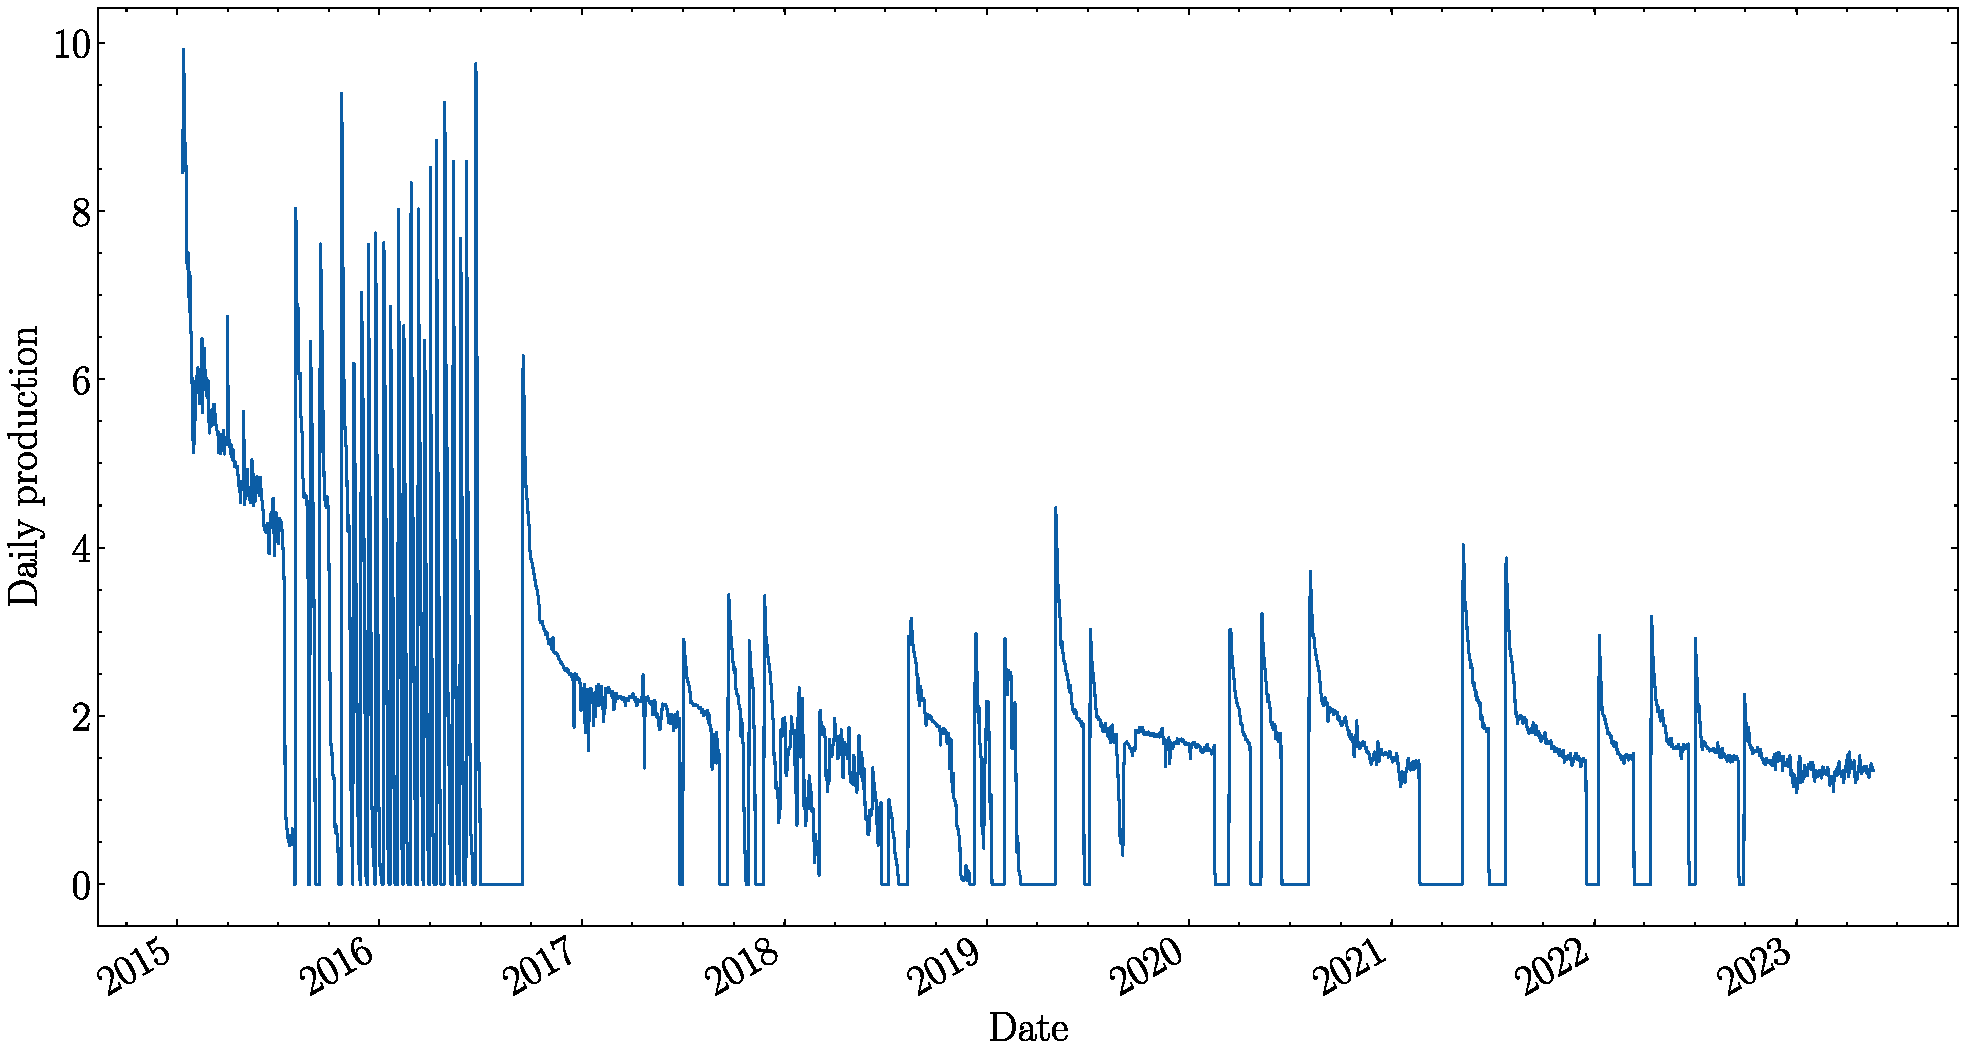
\includegraphics[width=.9\linewidth]{figure/DailyProduction_SN0004-04.pdf}
    \caption{井AA3876-NF的产量随时间的变化曲线}
    \label{fig:dailychange}
\end{figure}

在这套交互式图表中,用户将有能力选择特定的井来查看其产量变化,这使得用户能够专注于分析特定井的性能,同时也可以轻松切换查看其他井的产量数据。此外,这种交互式设计还允许用户检查曲线上每个点的具体值,从而获得详细的日产量信息。

通过这种交互式的数据可视化方法,用户不仅可以直观地观察每口气井随时间的产量变化,还可以有效比较不同井之间的产量差异,以及识别任何可能的异常或显著的趋势变化。这种分析工具将大大增强数据的可访问性和可理解性,为气井的管理和优化提供有价值的洞察。如图\ref{fig:dailychange}为
选取的井AA3876-NF的产量随时间的变化曲线。

% \begin{figure}[H]
%     \centering
%     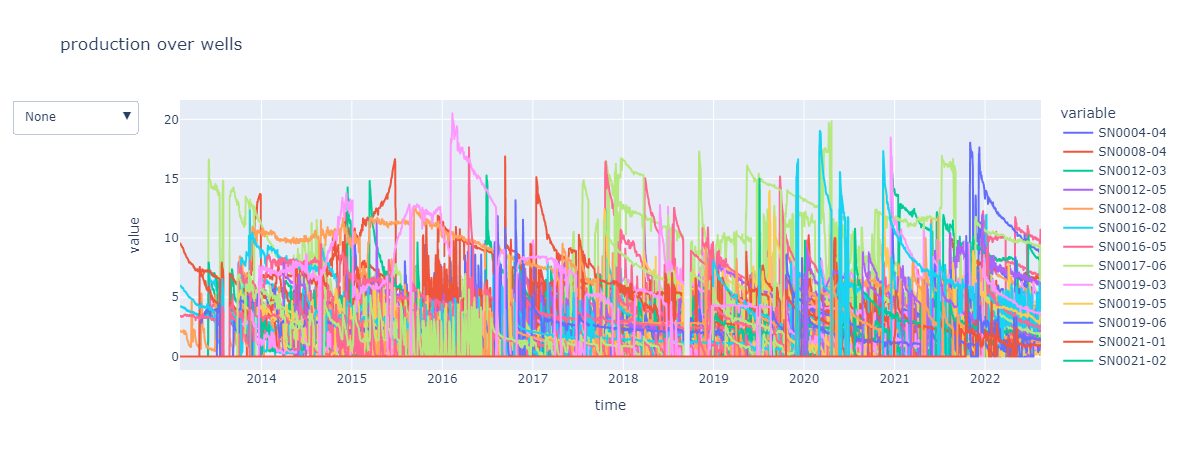
\includegraphics[scale=0.3,angle=0]{figure/productiongraph.png}
%     \caption{在一张图上同时绘制多口井产量随时间的变化曲线}
%     \label{fig:productionchange}
% \end{figure}
\subsection{RFM参数选取}
RFM模型对应的各组件为最近一次购买或交互(Recency)、购买或交互的频率(Frequency)、购买的货币价值(Monetary),是一种常用于客户价值分析的方法。
尽管它最初是为零售业和直接营销设计的,用于评估客户的购买行为,但其核心概念可以被扩展和应用于各种不同领域,包括能源产业等。在气井的背景
下,RFM模型可以被重新解释和调整,以评估气井的生产特性,具体如下:

Recency (R):最小开井近度。此指标反映了自气井上一次开井以来的时间跨度。在气井的运营过程中,最小开井近度作为衡量气井活跃度和响应速度的关键
指标。其公式如\eqref{eq:R}所示。
\begin{equation}
    R_i = t_{laset} - t_{i\_last}
    \label{eq:R}
\end{equation}
式中$t_{laset}$为用户定义的最后的截止日期,$t_{i\_last}$为气井最近一次的开井时间。i表示第i个气井。

Frequency (F):开井频度。该维度代表在特定时期内气井开井的频次。其公式如\eqref{eq:F}所示。
\begin{equation}
    F_i=\frac{N_{i\_days\_opend}}{N_{days\_sampled}}
    \label{eq:F}
\end{equation}
在这个公式中,如果备注中包含“open”一词,我们就计为1,否则计为0,然后将所有的1加起来,计算的到开井的日期。最后用开井日期除以样本总日期得到
最终的开井频度。

Monetary (M):平均开井产量。在传统RFM模型中代表消费金额,在气井场景中,这可以被理解为气井的生产量或产值,高产值的气井可能更具商业价值。其公式如
\eqref{eq:M}所示。
\begin{equation}
    M_i = \frac{mean(P_i)}{N_{i\_days\_opend}}
    \label{eq:M}
\end{equation}
其计算方式是将每个井i所有的日产气加起来,得到总的产气量$P_i$,然后除以开井时间。

通过综合考虑最小开井近度、开井时间和平均开井产量这三个维度,本文采用RFM模型对气井进行分类,旨在识别不同性能和潜力的气井群体。该方法不仅为气
井的综合评估提供了一种新的视角,而且通过量化分析支持了更为精准和个性化的气井管理策略的制定。此外,RFM模型的应用促进了对气井生产特性的深入理
解,为实现资源优化配置、提升生产效率以及最大化经济回报提供了坚实的分析基础。
\subsection{核密度估计}
使用RFM模型,并选定了合适的参数进行评估后。接下来需要通过基于核密度估计(KDE)方法来确定用于分类的阈值。核密度估计是一种估计概率密度函数的非参数方式,它可以从给定数据集出发,找到其概率分布的平滑估计。

本文选取的核函数为高斯核函数,具体如式\eqref{eq:gauss}所示。
\begin{equation}
    K(u) = \frac{1}{\sqrt{2\pi}} \exp\left(-\frac{1}{2} u^2\right)
    \label{eq:gauss}
\end{equation}
采用基于Silverman的规则(Silverman's rule of thumb)来计算带宽。具体公式如式\eqref{eq:silverman}所示。
\begin{equation}
    h = \left(\frac{4\hat{\sigma}^5}{3n}\right)^{\frac{1}{5}} \approx 1.06 \hat{\sigma} n^{-1/5}
    \label{eq:silverman}
\end{equation}
这里,\( n \) 表示样本大小,而 \( \hat{\sigma} \) 是样本的标准偏差。该公式为高斯核密度估计中带宽的选择提供了经验方法。

在确定了合适的核函数和带宽后,本文通过核密度估计,获得了一个连续的密度函数。得到的核密度函数进行Z-score归一化后的结果如图\ref{fig:KDE}所示。
\begin{figure}[H]
    \centering
    \subfloat[开井近度]{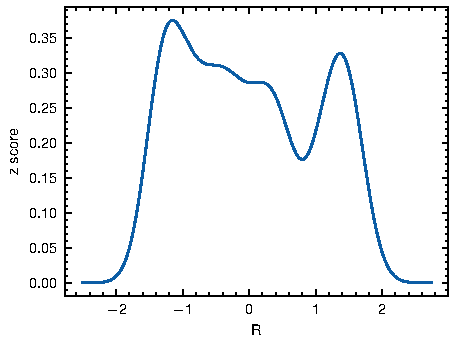
\includegraphics[width=.3\linewidth]{figure/R_z_kde.pdf}%
    \label{R}}
    \hfil
    \subfloat[开井频度]{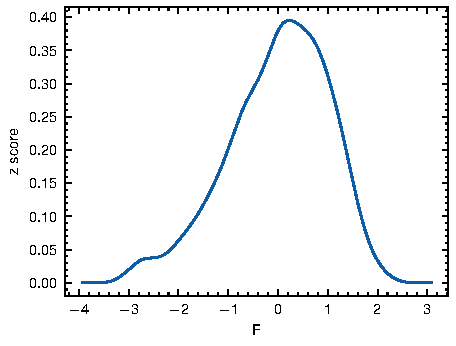
\includegraphics[width=.3\linewidth]{figure/F_z_kde.pdf}%
    \label{F}}
    \hfil
    \subfloat[平均开井产量]{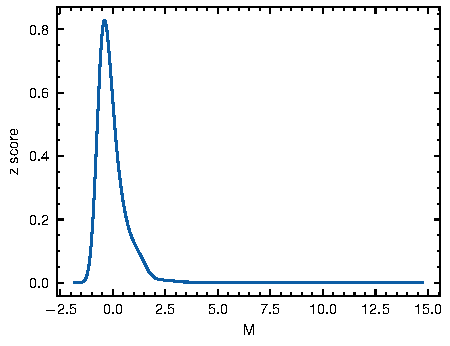
\includegraphics[width=.3\linewidth]{figure/M_z_kde.pdf}%
    \label{M}}
    \caption{核密度函数结果}
    \label{fig:KDE}
\end{figure}
\par
对于开井近度(R),由于其核密度估计结果呈现出两个明显的波峰,可以合理推断出有两种不同的工作状态。由于波谷处的开井近度较少见,可以作为两种不同工作模式的分界点,本文选取了两个波峰之间的波谷作为分类的阈值。位于左侧波峰的井被认为是近期频繁开井的,即开井
近度高;而位于右侧波峰的井则被视为近期较少开井,即开井近度低。这种分类有助于我们根据近期开井活动的频繁程度进行分析和管理。

开井频度(F)的分布呈现出接近正态分布的形态,表明大多数气井的开井频次集中在某个中间值附近,两端较少。这种分布反映了一个均衡的现象:既不频繁开关也不长时间不动作,维持了生产的稳定性和有效性。因此,对于开井频度,我们不设定特定的分类阈值,认为它遵循一种
普遍适用的操作规范。这种分布在企业的生产中也可以得到解释,如果开关频率过高,可能会造成气井反复积排液、增加摩阻损失、降低生产效率;但是如果开关频率过低,又导致底部水锥突破、增加水含率、降低天然气质量。因此其开关井频度会处于一种接近正态分布的形态。

最后,对于平均开井产量(M),其核密度估计结果显示在左侧有一个明显的峰值,而后向右平稳下降。这表明有一部分气井具有较高的平均开井产量,而其他气井的产量较低。据此,本文根据核密度估计的结果,以峰值右侧的起始下降点作为分类阈值,将平均开井产量的分布分为两类:高产量和低产量。
\begin{table}[H]
    \renewcommand{\arraystretch}{1.5}
    \centering
    \caption{气井分类模型及类型定义}
    \begin{tblr}{hlines, vlines,
        columns = {valign=m,co=-1},
        rows    = {halign=c},}
        开井近度 R  & 开井产量 M & 分类标准       & 生产价值类别   \\ 
        近         & 高        & 近高          & 活跃高价值 \\ 
        远         & 高        & 远高          & 不活跃高价值 \\ 
        近         & 低        & 近低          & 活跃一般价值 \\ 
        远         & 低        & 远低          & 不活跃一般价值 \\ 
    \end{tblr}
    % \begin{tabular}{|c|c|c|c|}
    % \hline
    % 开井近度 R  & 开井产量 M & 分类标准       & 生产价值类别   \\ \hline
    % 近         & 高        & 近高          & 活跃高价值 \\ \hline
    % 远         & 高        & 远高          & 不活跃高价值 \\ \hline
    % 近         & 低        & 近低          & 活跃一般价值 \\ \hline
    % 远         & 低        & 远低          & 不活跃一般价值 \\ \hline
    % \end{tabular}
    \label{table:KDE}
\end{table}

通过对开井近度和平均开井产量设定分类阈值,结合开井频度的分布特点,我们可以将气井分为四类,这样的分类有助于更精细地管理和调整生产策略,以提高整体生产效率和资源的有效利用。
具体如表\ref{table:KDE}所示。

通过以上步骤,将气井数据分为4类,每类气井具有不同的生产价值类型和KPI战术意义。对分类结果进行分析和评估,可以为气井的运营管理提供有针对性的建议。
例如,活跃高价值气井(近高)可以适当提高开井频度以充分发挥其生产潜力。活跃一般价值气井(近低)可通过实施工艺措施来提高开井产量等。

\section{本章小结}
本章介绍了对气井分类的必要性,分析了企业的气井不能使用普通聚类或者时间序列聚类的原因,随后引入了结合RFM与核密度估计的气井分类算法。本章展示了算法的框架,首先进行了数据清洗,将复杂的报表数据处理成可以直接进行数据操作的数据集。然后根据企业专家相关经验选取开井近度、开井频度和平均开井产量
作为RFM模型的参数,对选取后的参数通过核密度估计的方法来确定对其分类阈值。最终根据分类结果将气井分为四类井:活跃高价值气井、不活跃高价值气井、活跃一般价值气井和不活跃一般价值气井。通过这种方式来帮助企业对气井分类管理,接下来将根据分类结果在的产气量预测中分别执行预测算法。
% \section{分类结果}
% 最终对1000余口气井进行分类的结果如表\ref{fig:classtable}所示。
% \begin{table}[h]
%     \renewcommand{\arraystretch}{1.5}
%     \centering
%     \caption{每类气井类别数}
%     \label{fig:classtable}
%     \begin{tabular}{|c|c|}
%     \hline
%     分类 & 数量 \\ \hline
%     不活跃一般潜力    & 306 \\ \hline
%     活跃一般价值    & 228 \\ \hline
%     活跃一般潜力    & 149 \\ \hline
%     不活跃一般价值    & 122 \\ \hline
%     活跃高价值    & 99  \\ \hline
%     高潜力高价值    & 73  \\ \hline
%     可挖掘高价值  & 66  \\ \hline
%     不活跃高价值  & 31  \\ \hline
%     \end{tabular}
% \end{table}
    